\documentclass[twoside]{article}
\usepackage[a4paper]{geometry}
\geometry{verbose,tmargin=2.5cm,bmargin=2cm,lmargin=2cm,rmargin=2cm}
\usepackage{fancyhdr}
\pagestyle{fancy}

% nastavení pisma a~češtiny
\usepackage{lmodern}
\usepackage[T1]{fontenc}
\usepackage[utf8]{inputenc}
\usepackage[czech]{babel}

% odkazy
\usepackage{url}

\usepackage{float}
% vícesloupcové tabulky
\usepackage{multirow}
\usepackage{listings}
\usepackage{xcolor}
\usepackage{amssymb}
\usepackage{gensymb}
\usepackage{bbold}
\usepackage{amsmath}
\usepackage{siunitx}
\usepackage{mathtools}
\usepackage{commath}

% vnořené popisky obrázků
\usepackage{subcaption}

% automatická konverze EPS 
\usepackage{graphicx} 
\usepackage{epstopdf}
\epstopdfsetup{update}

\graphicspath{{./images}}

% odkazy a~záložky
\usepackage[unicode=true, bookmarks=true,bookmarksnumbered=true,
bookmarksopen=false, breaklinks=false,pdfborder={0 0 0},
pdfpagemode=UseNone,backref=false,colorlinks=true] {hyperref}


% Poznámky při překladu
\usepackage{xkeyval}	% Inline todonotes
\usepackage[textsize = footnotesize]{todonotes}
\presetkeys{todonotes}{inline}{}

%https://tex.stackexchange.com/questions/2783/bold-calligraphic-typeface
\DeclareMathAlphabet\mathbfcal{OMS}{cmsy}{b}{n}

% enumerate zacina s pismenem
\renewcommand{\theenumi}{\alph{enumi}}

% smaz aktualni page layout
\fancyhf{}
% zahlavi
\usepackage{titling}
\fancyhf[HC]{\thetitle}
\fancyhf[HLE,HRO]{\theauthor}
\fancyhf[HRE,HLO]{\today}
 %zapati
\fancyhf[FLE,FRO]{\thepage}

% údaje o autorovi
\title{OTE Domácí úkol 9 -- $\Sigma\Delta$ modulace}
\author{Vojtěch Michal}
\date{\today}

%customize code listing
\definecolor{codegreen}{rgb}{0,0.6,0}
\definecolor{codegray}{rgb}{0.5,0.5,0.5}
\definecolor{codepurple}{rgb}{0.58,0,0.82}
\definecolor{backcolour}{rgb}{0.95,0.95,0.92}

\lstdefinestyle{mystyle}{
    backgroundcolor=\color{backcolour},   
    commentstyle=\color{codegreen},
    keywordstyle=\color{magenta},
    numberstyle=\tiny\color{codegray},
    stringstyle=\color{codepurple},
    basicstyle=\ttfamily\footnotesize,
    breakatwhitespace=false,         
    breaklines=true,                 
    captionpos=b,                    
    keepspaces=true,                 
    numbers=left,                    
    numbersep=5pt,                  
    showspaces=false,                
    showstringspaces=false,
    showtabs=false,                  
    tabsize=2
}

\lstset{style=mystyle}

\begin{document}

\maketitle


Simulační schéma $\Sigma\Delta$ modulátoru je
zachyceno na obrázku \ref{schema}.
Jako vzorkovací signál je použit \textit{clock voltage}
o frekvenci 1 MHz.

\begin{figure}[h]
    \includegraphics[width=\textwidth]{schema.png}
    \caption{Simulační schéma}
    \label{schema}
\end{figure}
\clearpage
\section{Ověření funkce obvodu}


Po zkratování vstupů modulátoru byly zachyceny
průběhy na obrázku \ref{zkrat-vstupu}.
Je na nich patrná subharmonická složka na výstupu integrátoru.
Ta je způsobena faktem, že přepínání spínače S je řízeno na
konečné vzorkovací frekvenci. Tím pádem není střední hodnota
napětí integrátoru vždy dokonale nulová, ale
má tendenci driftovat od nuly. Když se naintegruje dostatečný offset,
jeden modulační cyklus vrátí střední hodnotu zpět k nule.

\begin{figure}[h]
    \includegraphics[width=\textwidth]{zkratovane_vstupy_zdaleka.png}
    \caption{Výstup integrátoru (modře) a klopného obvodu (červeně) při zkratovaném vstupu}
    \label{zkrat-vstupu}
\end{figure}


Detail signálů pro různé vstupní napětí je vidět na obrázkách 
\ref{0V}, \ref{95V} a \ref{-95V}.
Střída obdélníkového signálu na výstupu klopného obvodu je
dle očekávání 50 \% pro zkratované vstupy, a blízko k nule či jedničce
pro vstupní napětí blízko hranic rozsahu.


\begin{figure}
    \centering
    \begin{subfigure}{0.9\textwidth}
        
        \includegraphics[width=\textwidth]{0V.png}
        \caption{Pro $U_{\rm in} = \SI{0}{\volt}$.}
        \label{0V}
    \end{subfigure}

    \begin{subfigure}{0.45\textwidth}
        \includegraphics[width=\textwidth]{9,5V.png}
        \caption{Pro $U_{\rm in} = \SI{9.5}{\volt}$.}
        \label{95V}
    \end{subfigure}    
    \begin{subfigure}{0.45\textwidth}
        \includegraphics[width=\textwidth]{minus9,5.png}
        \caption{Pro $U_{\rm in} = \SI{-9.5}{\volt}$.}
        \label{-95V}
    \end{subfigure}
    \caption{Detail výstupu integrátoru (modře) a
    klopného obvodu (červeně) pro různá vstupní napětí $U_{\rm in}.$}
\end{figure}
\clearpage

\section{Převodní charakteristika}

Postupným připojením různých napětí v intervalu [-10, 10] V na vstup
modulátoru byla pomocí osciloskopu změřena závislost střídy výstupu
klopného obvodu na velikosti vstupního napětí. Změřené hodnoty jsou
uvedeny v tabulce \ref{tab:dc-sweep}. Srovnání s 
ideální lineární převodní charakteristikou je vykresleno na
obrázku \ref{chyba}.

\begin{table}[h]
    \centering
    \begin{tabular}{c|c}
        $U_{\rm in}$ [V] & střída výstupu klopného obvodu [\%] \\ \hline
        -9.5 & 2.54\\
        -7.5 & 12.37\\
        -5.0 & 24.85\\
        -2.5 & 37.61\\
        0.0 &  50.19\\
        2.5 & 62.40\\
        5.0 & 75.18 \\
        7.5 & 87.60\\
        9.5 & 97.52\\
    \end{tabular}
    \caption{Závislost střídy výstupu $\Sigma\Delta$ modulátoru na vstupním napětí}
    \label{tab:dc-sweep}
\end{table}

\begin{figure}[h]
    \centering
    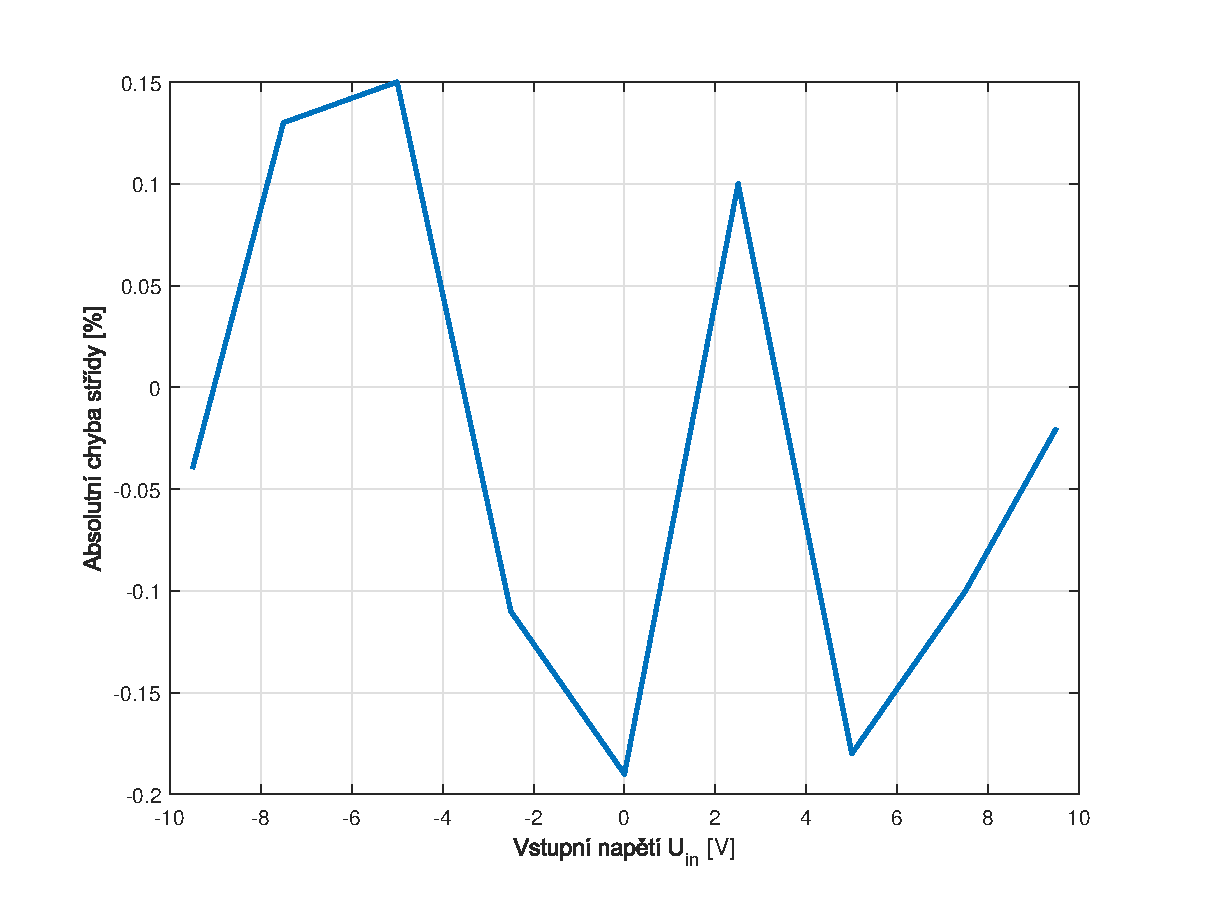
\includegraphics[width=0.8\textwidth]{chyba_prevodu.eps}
    \caption{Abolutní chyba střídy $\Sigma\Delta$ modulovaného signálu
    v závislosti na vstupním napětí}
    \label{chyba}
\end{figure}
\clearpage

\section{Harmonické vstupní signály}

Na vstup modulátoru byly přivedeny harmonické signály o frekvencích
1 Hz až 10 kHz 100 a 1000 Hz. Příslušné průběhy jsou vykresleny
na obrázkách \ref{harmonicke}.
Zeleně je vynesen vstupní harmonický signál, modře je výstup integrátoru.
Z deformací výstupu integrátoru v době, kdy je vsutpní signál v maximu,
je patrné, že $\Sigma\Delta$ modulátor má problémy pracovat
se vstupním napětím příliš blízkým hranicím rozsahu.
Pro vstupní frekvenci 10 kHz pak jsou již vidět značné deformace
kvůli klesajícímu poměru vstupní frekvence a modulační frekvence.

\begin{figure}[h]
    \centering
    \begin{subfigure}{0.45\textwidth}
        \includegraphics[width=\textwidth]{sin-10Hz.png}
        \caption{Pro $f_{\rm in} = \SI{10}{\hertz}$.}
        \label{10Hz}
    \end{subfigure}
    \begin{subfigure}{0.45\textwidth}
        \includegraphics[width=\textwidth]{sin-100Hz.png}
    \caption{Pro $f_{\rm in} = \SI{100}{\hertz}$.}
    \label{100Hz}
    \end{subfigure}
    \caption{Výstup integrátoru (modře) v závislosti na
    vstupním napětí (zeleně)}

    \begin{subfigure}{0.45\textwidth}
        \includegraphics[width=\textwidth]{sin-1000Hz.png}
        \caption{Pro $f_{\rm in} = \SI{1}{\kilo\hertz}$.}
        \label{1000Hz}
    \end{subfigure}
    \begin{subfigure}{0.45\textwidth}
        \includegraphics[width=\textwidth]{sin-10000Hz.png}
    \caption{Pro $f_{\rm in} = \SI{10}{\kilo\hertz}$.}
    \label{10000Hz}
\end{subfigure}
\caption{Výstup integrátoru (modře) v závislosti na
vstupním napětí (zeleně)}
\label{harmonicke}
\end{figure}

\end{document}

